\documentclass[conference]{IEEEtran}
\IEEEoverridecommandlockouts
\usepackage{cite}
\usepackage{amsmath,amssymb,amsfonts}
\usepackage{graphicx}
\usepackage{booktabs}
\usepackage{array}
\usepackage{url}
\usepackage{xcolor}
\usepackage{balance}

\begin{document}

\title{Secure Online Gaming Platform: Detection and Mitigation of Cheating and Account Breaches}

\author{\IEEEauthorblockN{Sudarshan J N, Varun Kumar L, Prajwal K And Dileep}
\IEEEauthorblockA{Department of Computer Science and Engineering\\
PES University, Electronic City Campus\\
Bengaluru, India}}

\maketitle

\begin{abstract}
Online first-person shooter games are exposed to unfair gameplay behaviors that can affect competitive integrity and player trust. Detecting such behavior is challenging because suspicious actions may resemble legitimate high-skill play, while isolated events rarely provide sufficient evidence for a reliable decision. This paper presents SecureFPS, a security-oriented online FPS platform that combines gameplay telemetry, server-side monitoring, role-based administration, and machine-learning-assisted behavioral analysis. The detection workflow uses a calibrated supervised Random Forest classifier together with an Isolation Forest anomaly detector and a 60/40 weighted risk score. The platform architecture, feature pipeline, model outputs, dashboard workflow, security controls, and evaluation methodology are described. On the project's held-out benchmark, the Random Forest evaluation achieved 0.9145 precision, 0.8580 recall, 0.8854 F1-score, and 0.9729 ROC-AUC. The Isolation Forest evaluation reported 0.9791 precision and 0.3219 recall under its benchmark operating convention. These measurements characterize the supplied dataset and do not establish guaranteed real-world effectiveness; model detections remain review evidence rather than proof of misconduct.
\end{abstract}

\begin{IEEEkeywords}
Online games, first-person shooter, gameplay telemetry, cheat detection, Random Forest, Isolation Forest, anomaly detection, behavioral analysis, risk scoring.
\end{IEEEkeywords}

\section{Introduction}
Online multiplayer first-person shooter (FPS) games require players to compete under a shared set of game rules. Unfair tools or abnormal gameplay behavior can undermine match outcomes and reduce confidence in the game environment. Conventional rule-based detection can identify some known violations, but it may be less effective when suspicious behavior changes over time or when individual actions are not independently conclusive.

A behavioral detection system can complement conventional game-server validation by examining patterns across multiple gameplay events. Examples include unusually consistent aiming, atypical firing patterns, improbable hit behavior, and movement patterns that differ from expected gameplay. However, these signals must be interpreted carefully. High accuracy or a high kill count alone does not establish cheating, because player skill, weapon choice, latency, map geometry, and match context can affect observed statistics.

SecureFPS is designed as an online FPS platform with player-facing gameplay and account features, administrator monitoring, persistent data storage, and a machine-learning-assisted security workflow. The project context includes a game client, a web dashboard, a Flask-based service layer, MongoDB persistence, and real-time communication through Socket.IO. The exact deployed versions and final module boundaries must be confirmed against the current source tree before submission.

The main contributions of this draft are:
\begin{itemize}
    \item A platform-level design that connects gameplay events, server-side telemetry processing, persistence, and administrative monitoring.
    \item A division of responsibilities between supervised classification using Random Forest and unsupervised anomaly detection using Isolation Forest.
    \item A transparent risk-index formulation that keeps model outputs distinguishable from a calibrated probability of cheating.
    \item A security and evaluation framework that emphasizes authoritative match summaries, access control, reproducibility, and honest reporting of unavailable measurements.
\end{itemize}

\section{Related Work}
Random Forest is an ensemble learning method that combines the outputs of multiple decision trees. It is widely used for classification and regression because it can model nonlinear relationships and interactions among input features while reducing the variance associated with an individual tree \cite{breiman2001}.

Isolation Forest approaches anomaly detection by isolating observations through randomly selected features and split values. Anomalies tend to be isolated using shorter paths than ordinary observations, allowing an anomaly score to be derived from average path length \cite{liu2008}. Unlike a supervised classifier, the method does not require every training observation to have a normal or cheating label.

These methods provide complementary signals. A supervised model can learn patterns represented in labelled examples, while an unsupervised detector can flag unusual observations that may not match known labelled patterns. Neither method independently establishes intent or proves a rule violation. SecureFPS therefore treats model outputs as review signals that should be interpreted alongside match context and validated server events.

\section{System Overview}
\subsection{Architecture}
The intended SecureFPS workflow is organized into five logical layers:
\begin{enumerate}
    \item \textit{Game client:} captures gameplay actions and presents the game interface and HUD.
    \item \textit{Real-time communication:} transports permitted gameplay and match events between clients and the server.
    \item \textit{Backend services:} validate requests, enforce authentication and authorization, apply match rules, and process telemetry.
    \item \textit{Data and model layer:} stores user, match, and telemetry records and invokes the trained detection models.
    \item \textit{Web dashboards:} present player information and authorized monitoring information to administrators.
\end{enumerate}

\begin{figure*}[t]
\centering
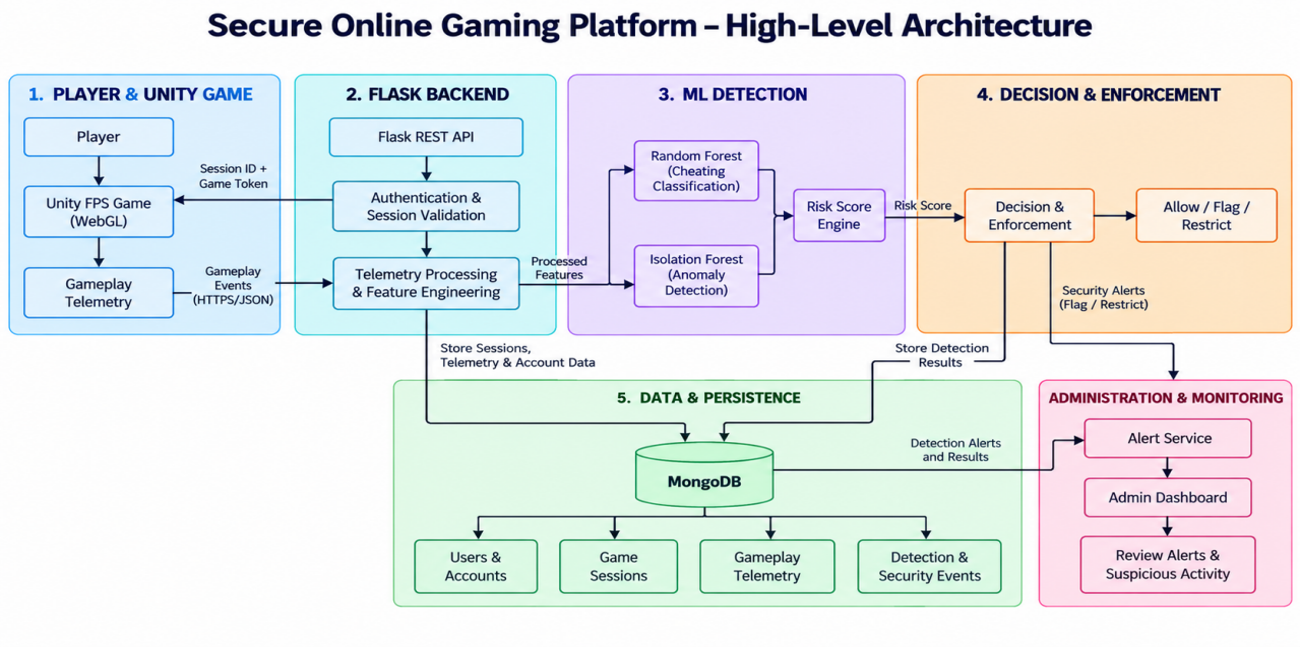
\includegraphics[width=0.98\textwidth]{architecture.png}
\caption{High-level architecture of the SecureFPS platform.}
\label{fig:architecture}
\end{figure*}

Fig.~\ref{fig:architecture} summarizes the logical flow. The game client is not treated as the authority for security-sensitive outcomes. Where possible, the backend should validate match state and event ownership before accepting telemetry for statistics or detection. A dashboard should display only records that the authenticated user is permitted to access.

\subsection{Roles and Access Control}
The platform distinguishes player, normal-administrator, and super-administrator responsibilities. Players access their own profile, match history, and gameplay-related information. Normal administrators perform only the moderation and monitoring operations granted by their saved permissions. Super administrators manage privileged configuration and system-level functions. Authorization must be enforced by backend routes and real-time event handlers; hiding a button in the frontend is not sufficient protection.

Authentication-related operations include password verification, account restrictions, optional multi-factor authentication, recovery, session expiry, logout, and revocation. State-changing web requests should use the application's CSRF protections. Sensitive credentials, password hashes, MFA secrets, recovery tokens, and session tokens must never be included in dashboard responses or exported telemetry.

\section{Gameplay Telemetry and Feature Processing}
\subsection{Telemetry Collection}
The detection workflow can use event-level information generated during a match. Candidate telemetry includes movement distance and direction, velocity changes, aiming adjustments, firing timestamps, weapon information, hit outcomes, headshot outcomes where available, and match identifiers. The final feature set must be restricted to fields that are actually captured, validated, and persisted by the implementation.

A telemetry record should be associated with a player, match, event time, and event type. The server should reject events that do not belong to the active session or valid match state. Duplicate event delivery must be handled idempotently so that reconnects or network retries do not inflate shot, hit, kill, or headshot counts.

\subsection{Feature Extraction}
Raw events are transformed into a feature vector for a defined observation window. Depending on the available implementation, derived features may include shots per interval, hit ratio, headshot ratio, firing interval variability, aim-change magnitude, movement speed, movement-direction changes, and ratios between observed actions. These are candidate feature definitions, not a claim that every feature is currently implemented.

Let the feature vector for player $u$ in observation window $t$ be
\begin{equation}
\mathbf{x}_{u,t}=[x_1,x_2,\ldots,x_m]^T,
\label{eq:featurevector}
\end{equation}
where $m$ is the number of validated features. Training and inference must use the same feature order, units, missing-value policy, and preprocessing steps. Features that are unavailable for a historical match should be marked as missing rather than silently replaced with values that imply normal behavior.

\subsection{Authoritative Match Statistics}
For a player with $S$ valid shots and $H$ successful hits, career accuracy is computed from aggregate totals:
\begin{equation}
\mathrm{Accuracy}(\%)=\begin{cases}
100\dfrac{H}{S}, & S>0,\\
\text{Unavailable}, & S=0.
\end{cases}
\label{eq:accuracy}
\end{equation}
The kill/death ratio is
\begin{equation}
\mathrm{K/D}=\begin{cases}
\dfrac{K}{D}, & D>0,\\
K, & D=0,
\end{cases}
\label{eq:kd}
\end{equation}
where $K$ is the kill count and $D$ is the death count. The zero-death convention must be stated consistently in the user interface. An alternative convention may be selected, but division by zero must never occur. Match-level authoritative summaries should be resolved before career aggregation to prevent duplicate counting.

\section{Machine-Learning Detection Models}
\subsection{Random Forest Classification}
Random Forest is a supervised ensemble classifier. During training, multiple decision trees are built using randomized training samples and feature subsets. Each tree learns decision rules that partition the feature space. At inference time, the trees vote for a class, and the ensemble returns the class with the largest vote count.

Let $T$ be the number of trees and $h_j(\mathbf{x})$ be the class predicted by tree $j$. The ensemble class is
\begin{equation}
\hat{y}_{RF}(\mathbf{x})=\operatorname{mode}\{h_1(\mathbf{x}),\ldots,h_T(\mathbf{x})\}.
\label{eq:rfclass}
\end{equation}
For a binary model, labels may be encoded as 0 and 1. The semantic meaning of each label must be taken from the actual training-label mapping. In this paper, the notation $y=1$ denotes the suspicious class and $y=0$ denotes the normal class for the proposed formulation; this mapping must be changed if the project's dataset uses the reverse encoding.

When the trained implementation supports probability estimates, the suspicious-class vote proportion can be represented as
\begin{equation}
p_{RF}(\mathbf{x})=\frac{1}{T}\sum_{j=1}^{T} I(h_j(\mathbf{x})=1),
\label{eq:rfprob}
\end{equation}
where $I(\cdot)$ is the indicator function. The corresponding percentage is $100p_{RF}$. In common machine-learning libraries, a probability estimate may be obtained using a method such as \texttt{predict\_proba}; the class column must be selected using the model's class ordering, not by assuming that column 1 always means suspicious.

A predicted label of 1 is a classification decision. A value such as $p_{RF}=0.80$ is a model score or estimated class probability, not automatically an 80\% real-world probability that the player is cheating. Calibration and evaluation on representative held-out data are required before interpreting it probabilistically.

\subsection{Isolation Forest Anomaly Detection}
Isolation Forest is an unsupervised anomaly-detection method. It constructs isolation trees by repeatedly selecting a feature and a split value. Observations that differ substantially from the majority of the training data tend to be isolated after fewer splits. The average path length across trees is used to derive an anomaly score.

For a sample $\mathbf{x}$ and subsample size $n$, the standard Isolation Forest score is
\begin{equation}
s(\mathbf{x},n)=2^{-\frac{E[h(\mathbf{x})]}{c(n)}},
\label{eq:ifscore}
\end{equation}
where $E[h(\mathbf{x})]$ is the average path length and $c(n)$ is the average path length of an unsuccessful search in a binary search tree:
\begin{equation}
c(n)=2H(n-1)-\frac{2(n-1)}{n},
\label{eq:cn}
\end{equation}
with $H(i)$ denoting the $i$-th harmonic number. Under this standard formulation, scores closer to 1 indicate more anomalous observations, scores near 0.5 are near the expected baseline, and smaller scores generally indicate ordinary observations.

Implementations such as scikit-learn expose methods including \texttt{score\_samples}, \texttt{decision\_function}, and \texttt{predict}. Their sign and threshold conventions differ from the standard score in \eqref{eq:ifscore}. In scikit-learn, \texttt{predict} commonly returns 1 for inliers and -1 for outliers, while lower \texttt{score\_samples} values are more abnormal. Therefore, the project must explicitly transform the library output before displaying a higher-is-riskier score. Isolation Forest does not directly estimate a calibrated probability of cheating.

\subsection{Combined Risk Index}
The two models provide different evidence: Random Forest estimates similarity to labelled suspicious examples, while Isolation Forest measures deviation from the learned distribution of observations. A combined score can be defined after mapping both signals to a common range.

Let $r_{RF}\in[0,1]$ be the Random Forest suspicious-class score, and let $r_{IF}\in[0,1]$ be the normalized Isolation Forest anomaly score, where larger values consistently indicate greater concern. A weighted index is
\begin{equation}
R=100\left(\alpha r_{RF}+(1-\alpha)r_{IF}\right),
\label{eq:risk}
\end{equation}
where $0\leq\alpha\leq1$. The weight $\alpha$ must be selected using validation experiments and documented with the model version. If an anomaly score is transformed from a library-specific output, the transformation and its calibration range must be reported. The score $R$ is a risk index, not a probability of cheating.

For illustration only, suppose $r_{RF}=0.80$, $r_{IF}=0.60$, and a validation-selected weight is $\alpha=0.60$. Then
\begin{equation}
R=100[(0.60)(0.80)+(0.40)(0.60)]=72.
\end{equation}
This example demonstrates the arithmetic only. The values and weight are not measured SecureFPS results and must not be presented as the project's deployed configuration unless confirmed by source code and experiments.

If either model is unavailable, the system should not silently substitute zero. It should mark the combined score as incomplete or unavailable, or use an explicitly documented partial-evidence policy. A final category such as low, medium, or high risk requires thresholds selected using validation data and an acceptable false-positive trade-off. Model output should initiate review rather than an automatic ban unless a separately specified, validated policy authorizes such an action.

\section{Dashboard and Data Presentation}
The player dashboard is intended to show account information, match history, and statistics derived from persisted match summaries. The normal-administrator dashboard is intended to show authorized player monitoring, match records, alerts, and review requests. The super-administrator dashboard may expose system configuration, role management, model lifecycle information, and operational status. The final set of panels must match the working application; a planned or placeholder panel must not be described as a functioning feature.

Every dashboard value should be traceable to its source. A displayed statistic should identify whether it is stored, calculated from persisted records, generated by a model, or measured from a live service. For example, career accuracy should be calculated from total successful hits divided by total valid shots, not by averaging match percentages. A model-performance panel should use an actual evaluation result tied to a model version and test dataset. A service-health panel should report a real health check or show an unavailable state.

The frontend should distinguish at least four states: available data, empty data, incomplete data, and unavailable service. An API failure must not be converted into a successful-looking zero value. Role-specific APIs must enforce ownership and permissions on the server. Exported records must exclude credentials and other authentication secrets.

\section{Implementation Considerations}
The project context identifies a web backend, MongoDB persistence, real-time gameplay communication, and a browser-based dashboard. A practical implementation should keep route handlers, business logic, model inference, and database access separated sufficiently to test them independently. The model-loading path should fail visibly and safely if a model artifact is missing or incompatible.

Database records should use stable identifiers and explicit ownership fields. Indexes should support common queries such as player match history, match event retrieval, and time-bounded telemetry analysis. Writes that affect balances, purchases, rewards, or match summaries should be idempotent where retries are possible. Multiplayer hit events should have unique event identifiers or another deduplication mechanism.

The authoritative match result should be finalized once, after validating the match termination condition. For the specified Bot Combat and multiplayer modes, the intended termination condition is 15 kills or 480 seconds, whichever occurs first. The server, HUD, results view, restart, and rematch flows should use the same rule. Training and Free Roam should retain their separate behavior.

\section{Experimental Methodology and Evaluation Plan}
A reproducible evaluation should be conducted using a dataset that is separated by player or match where possible, reducing leakage between training and test partitions. Randomly splitting individual telemetry rows can overestimate generalization if records from the same player or match appear in both partitions.

For Random Forest, report the class distribution, feature list, preprocessing, train/validation/test split, hyperparameters, random seed, confusion matrix, precision, recall, F1-score, and ROC-AUC where appropriate. Report class-specific performance because false positives may unfairly flag legitimate players. If probabilities are displayed as probabilities, include a calibration assessment such as reliability analysis or Brier score.

For Isolation Forest, report the training population, feature preprocessing, contamination setting, threshold-selection method, and anomaly-detection performance against a labelled evaluation set if labels are available. The contamination parameter is an assumption about the expected proportion of anomalies in the fitting data; it is not a guaranteed real-world cheating rate.

Table~\ref{tab:results} reports the measured results from the project's held-out evaluation and benchmark reports.

\begin{table}[t]
\caption{Measured SecureFPS Model Evaluation Results}
\label{tab:results}
\centering
\scriptsize
\setlength{\tabcolsep}{3pt}
\resizebox{\columnwidth}{!}{%
\begin{tabular}{lcc}
\toprule
\textbf{Metric} & \textbf{Random Forest} & \textbf{Isolation Forest}\\
\midrule
Test samples & 576 & 676\\
Precision & 0.9145 & 0.9791\\
Recall & 0.8580 & 0.3219\\
F1-score & 0.8854 & 0.4845\\
ROC-AUC & 0.9729 & 0.8085\\
False-positive rate & 0.0314 & Reported as precision/recall basis\\
\bottomrule
\end{tabular}}
\end{table}

In addition to model metrics, system evaluation should measure inference latency, event-processing throughput, database write latency, and dashboard update delay under controlled load. These are system measurements and must be collected from repeatable tests rather than estimated or hardcoded.

\section{Limitations and Threats to Validity}
Behavioral detection is sensitive to dataset quality, class imbalance, player skill variation, weapon characteristics, map design, network latency, and changes in game mechanics. A model trained on one game version may become less reliable after gameplay changes. Attackers may also adapt their behavior to avoid learned patterns.

A risk index can be misleading if its component scores are not normalized consistently or if its weights are selected without validation. A model probability is not necessarily calibrated, and an anomaly score is not a probability. Incomplete telemetry, client-side manipulation, duplicate events, and incorrect player-to-match association can corrupt both detection and dashboard statistics. Server-side validation, auditability, and human review remain important safeguards.

This draft reflects the supplied IEEE template and inspection of the project implementation and model reports. Remaining items for final submission include confirmation of the dataset provenance, reporting of the exact training and test partitions, and collection of independent real-player and adversarial evaluation measurements before operational deployment.

\section{Conclusion and Future Work}
This paper presented SecureFPS as a telemetry-driven online FPS security framework that combines gameplay monitoring, persistent match data, role-based dashboards, and complementary machine-learning techniques. Random Forest provides supervised classification based on labelled examples, while Isolation Forest identifies unusual observations without requiring every training sample to be labelled. A weighted risk index can combine the two signals, provided that score direction, normalization, weights, and thresholds are validated and documented.

Future work includes completing source-level traceability for every telemetry feature and dashboard value, collecting representative gameplay data, evaluating both models on leakage-resistant test partitions, calibrating model outputs where probability interpretation is required, and measuring runtime performance. The system should continue to treat model detections as evidence for investigation rather than conclusive proof of misconduct.

\section*{Acknowledgment}
The author may add acknowledgments for project supervision, institutional support, datasets, or other contributions here. Remove this section if it is not applicable.

\balance
\begin{thebibliography}{00}
\bibitem{breiman2001}
L. Breiman, ``Random forests,'' \emph{Machine Learning}, vol. 45, no. 1, pp. 5--32, 2001, doi: 10.1023/A:1010933404324.

\bibitem{liu2008}
F. T. Liu, K. M. Ting, and Z.-H. Zhou, ``Isolation forest,'' in \emph{Proc. IEEE International Conference on Data Mining}, 2008, pp. 413--422, doi: 10.1109/ICDM.2008.17.

\bibitem{scikit}
F. Pedregosa \emph{et al.}, ``Scikit-learn: Machine learning in Python,'' \emph{Journal of Machine Learning Research}, vol. 12, pp. 2825--2830, 2011.

\bibitem{ieeetran}
M. Shell, ``How to use the IEEEtran \LaTeX\ class,'' IEEEtran documentation, 2015.
\end{thebibliography}

\end{document}
